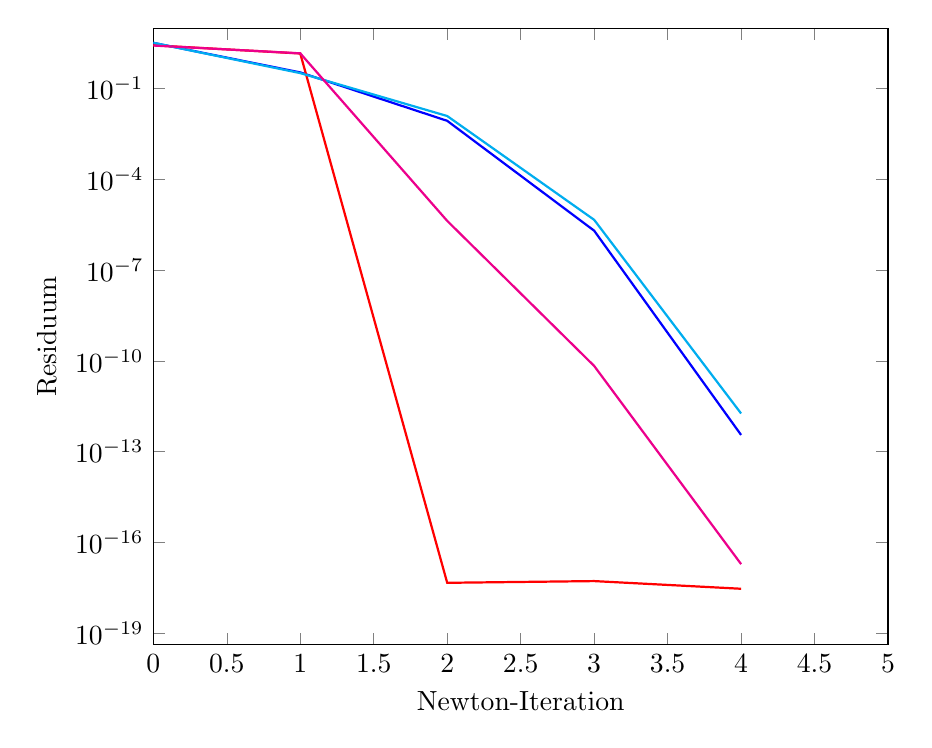
\begin{tikzpicture}[every plot/.append style={thick}] 
\begin{axis}[ 
label style={font=\normalsize}, 
xlabel={Newton-Iteration}, 
ylabel={Residuum}, 
xmin=0, xmax=5, 
ymode=log, 
ymin=0, ymax=10, 
width=0.9\textwidth, 
grid style=dashed, 
] 
\addplot[ 
color=blue, 
] 
coordinates { 
(0, 3.29e+00)(1, 3.46e-01)(2, 8.68e-03)(3, 2.02e-06)(4, 3.55e-13)}; 
\addplot[ 
color=red, 
] 
coordinates { 
(0, 2.73e+00)(1, 1.46e+00)(2, 4.58e-18)(3, 5.22e-18)(4, 2.91e-18)}; 
\addplot[ 
color=cyan, 
] 
coordinates { 
(0, 3.30e+00)(1, 3.28e-01)(2, 1.25e-02)(3, 4.62e-06)(4, 1.82e-12)}; 
\addplot[ 
color=magenta, 
] 
coordinates { 
(0, 2.68e+00)(1, 1.48e+00)(2, 4.26e-06)(3, 6.81e-11)(4, 1.90e-17)}; 
\end{axis} 
\end{tikzpicture} 
